%!TEX root = ../main.tex
 \section{強化学習の実践}

 本節では,強化学習を用いて問題を解くAIを作成する方法を学ぶ.

 まず最初に,与えられた単純な迷路に対して報酬を最大化するAIを,単純なQ学習を用いて作ることで,強化学習の基礎を理解する.その後に,ChainerRLを用いて実践的なAIを作り,複雑な問題に対して強化学習を適用する方法を学ぶ.

  \subsection{準備}

  最初のタスクは,単純な迷路である.図\ref{fig:env1}に示す2次元の離散的な空間(グリッドワールド)において,スタートからゴールを目指すことが目標となる.図\ref{fig:env1}において,エージェントはSと書かれた位置($(y, x) = (0, 0)$)から行動を始め,Gと書かれた位置($(y, x) = (2, 3)$)にたどり着くことを目指す.エージェントは4方向に動くことができるが,灰色で表されるマスには侵入できない(移動できず1stepが経過する).エージェントは迷路全体を観測することはできず,自分のいる$x, y$座標を観測することができる.

  \begin{figure}[htb]
   \centering
   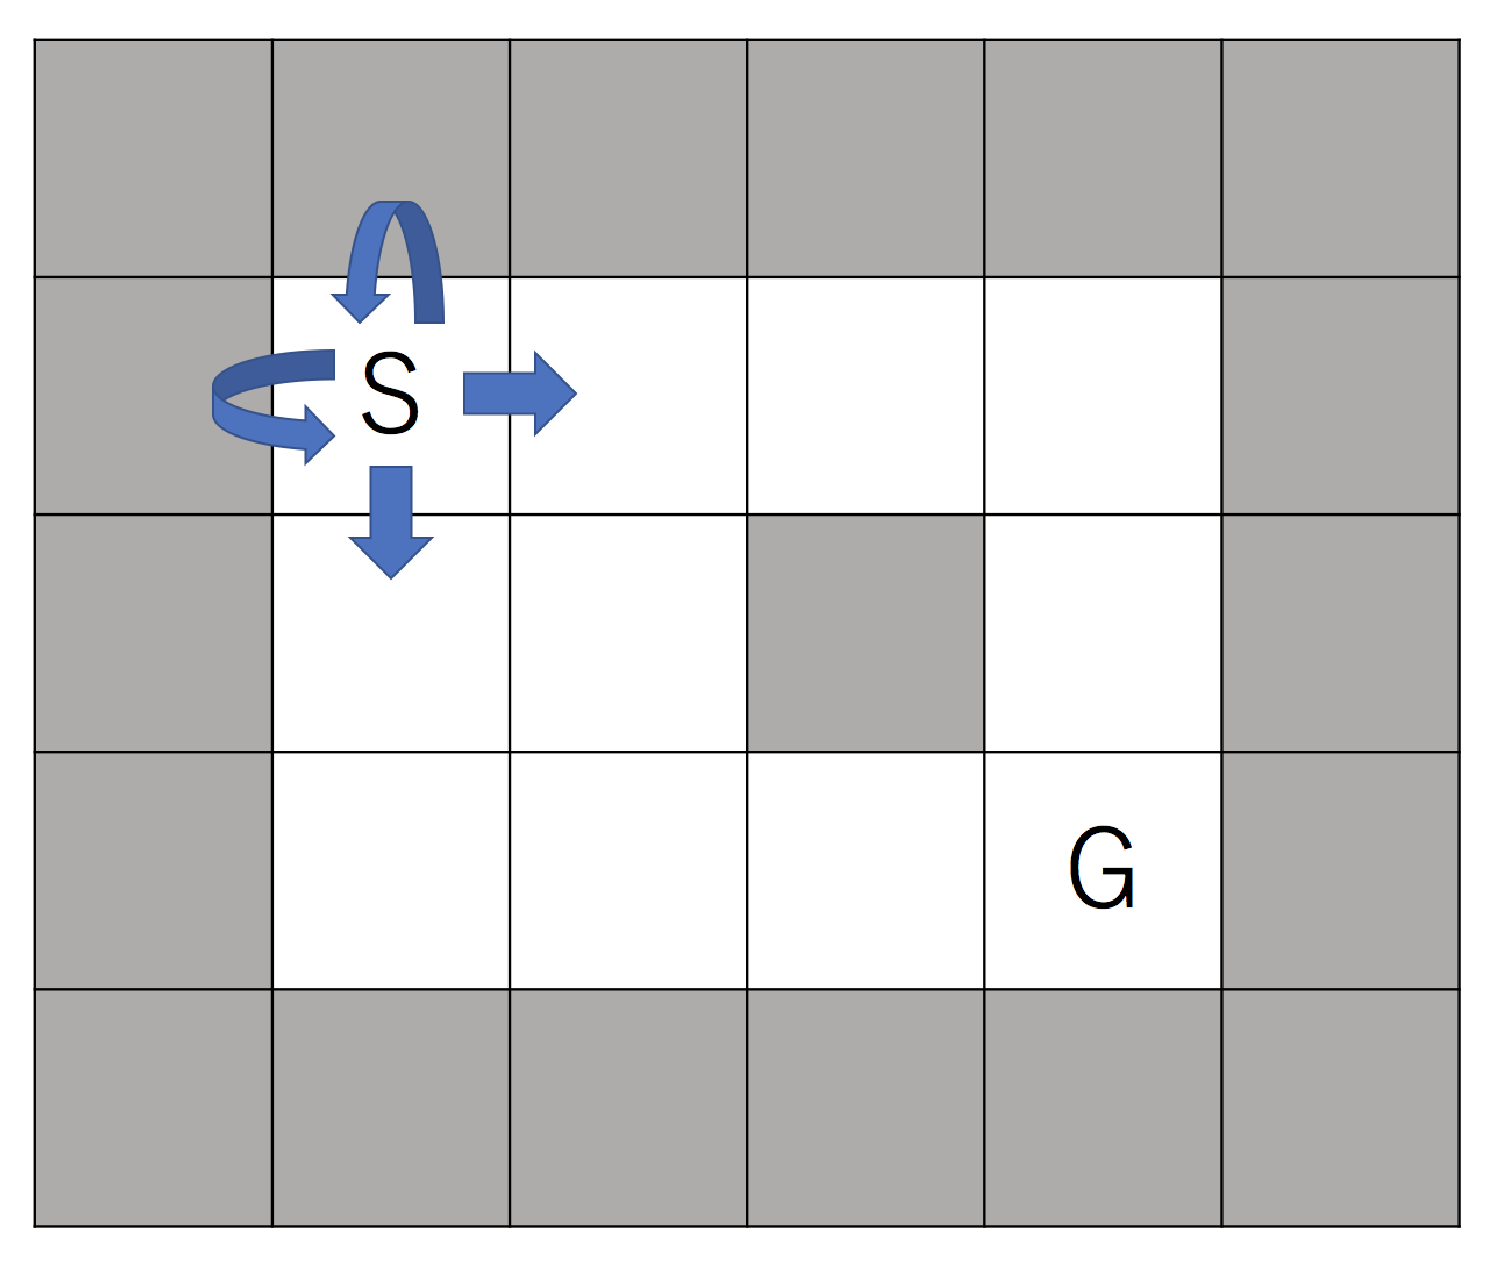
\includegraphics[width=80mm]{images/TsuruokaLab/env1.eps}
   \caption{単純な迷路}
   \label{fig:env1}
  \end{figure}

  \verb+dl_exp_rl.tar.gz+を展開してソースコードを入手しよう.ソースコードの中にある\verb+main.py+を実行することで,ランダムに動くエージェントが迷路に取り組む様子が観察できる.

  \newpage

   %$wget --http-user=dlexp --http-passwd=dlexp http://www.logos.ic.i.u-tokyo.ac.jp/~kkawamura/dl_exp/dl_exp_rl.tar.gz
  \begin{lstlisting}[basicstyle=\ttfamily\footnotesize, frame=single]
   $tar xzvf dl_exp_rl.tar.gz
   $cd dl_exp_rl
   $python main.py
  \end{lstlisting}


  \begin{practice}
   ソースコードをダウンロードし,\verb+main.py+を実行せよ.
   また,\verb+README.md+を読み,\verb+random_agent.py+ と \verb+easymaze_env.py+ の場所を確認せよ.
  \end{practice}

  迷路の様子が標準出力に一気に流れ込んでくるので,少し眺めたら\verb-Ctrl+c-で止めてしまって構わない.
  また,ゆっくり眺めたければ
  \begin{lstlisting}[basicstyle=\ttfamily\footnotesize, frame=single]
   $python main.py | less
  \end{lstlisting}
  のようにすればよい.

  \subsection{相互作用の理解}
  このタスクに限らず,強化学習は環境とエージェントが相互作用することで学習を行うものである.

  今回用いるソースコードは,オープンソースライブラリであるOpenAI Gym (\url{https://github.com/openai/gym}) ,およびChainerRL (\url{https://github.com/chainer/chainerrl}) の書式に則って書かれており,環境とエージェントが完全に分かれている.その二者の相互作用を担うのが\verb+main.py+である.

  \verb+main.py+を読み,適宜編集・実行しつつ,エージェントと環境がどのように相互作用しているのかを理解しよう.

  \begin{practice}
   \verb+main.py+の中で,envおよびagentを作成している行を答えよ.
   また,これらに対して呼び出されているインスタンス変数・メソッドをすべて挙げよ.
   自由課題などでenvやagentを自分で作成する場合,最低限これらの変数・メソッドをすべて実装する必要がある(インタフェース).
  \end{practice}

  演習の解答は\verb+answer_sheet.md+に書き込むとよい.

  なお,\verb+main.py+内の\verb+prints_detail+変数を\verb+False+にすることで,毎stepの迷路の出力を止めることができる.

  \begin{practice}
   \label{practice:100episodes}
   train, testのそれぞれで100 episodes の実験を行って,ランダムエージェントがゴールするまでのepisodeごとの平均step数を出力せよ.\verb+main.py+の編集が必要となる.
   300 steps 掛かってもゴールできない場合,300 steps でゴールしたものとして平均を計算せよ.
  \end{practice}

  episodeごとの平均rewardは既に出力されるようになっているので,その実装を参考にするとよい.

  \subsection{エージェントの理解}
  \label{subsec:rulebase}
  \verb+random_agent.py+を読み,ランダムエージェントがどのように動作しているかを理解しよう.

  ランダムエージェントは,\verb+__init__()+で行動集合のサイズを取得し,\verb+act()+が呼び出されると行動の中から一つをランダムに選ぶようになっている.

  ランダムエージェントはこの小さな迷路でもゴールするのにかなり時間がかかってしまうが,迷路の形状は毎回同じなので,人間であればすぐに最短経路を求めることができるはずである.

  例えば,「壁にぶつかるまで下に行き,ぶつかったら右に行く」などはその一例である.

  \begin{practice}
   \label{practice:rulebase}
   コメントを参考に,穴あきファイル\verb+rulebase_agent.py+の穴を埋めることで,この形状の迷路を最短step数で解くルールベースエージェントを作成せよ.「壁にぶつかるまで下に行き,ぶつかったら右に行く」ように実装すればよい.
   エージェントが受け取る観測を,\verb+print()+関数を用いたり\verb+easymaze_env.py+を読んだりすることで確認することが必要となることに注意せよ.
  \end{practice}

  \verb+main.py+の
  \begin{lstlisting}[basicstyle=\ttfamily\footnotesize, frame=single]
   agent = agents.RandomAgent(env, gpu_id)
  \end{lstlisting}
  を
  \begin{lstlisting}[basicstyle=\ttfamily\footnotesize, frame=single]
   agent = agents.RulebaseAgent(env, gpu_id)
  \end{lstlisting}
  に変更するだけで,ランダムエージェントの代わりにルールベースエージェントを試すことができる.

  また,\verb+rulebase_agent.py+内の
  \begin{lstlisting}[basicstyle=\ttfamily\footnotesize, frame=single]
   raise NotImplementedError()
  \end{lstlisting}
  は,「このセクションはまだ実装されていないので,ここを通るときは必ず実行時エラーを出してください」という合図である.穴を埋めた後はこの行を削除すればよい.


  \subsection{環境の理解}
  演習\ref{practice:rulebase}で作成したように,人間が迷路を観察し,あらかじめ移動ルールを定めておくことで,単純な迷路を解くAIは作成できる.

  しかしながら,この方法では異なる環境に対応できない.\verb+easymaze_env.py+を編集し,これを示そう.

  \begin{practice}
   \verb+easymaze_env.py+を編集し,迷路に最小限の変更を行うことで,演習\ref{practice:rulebase}で作成したエージェントがゴールできないような環境にせよ.ただし,別のルートでゴールできるようにしておくこと.
  \end{practice}

  この章ではあまり詳しく触れないが,自由課題で自作の環境に対して強化学習を適用したい場合,このソースコードを基に各メソッドを定義するとよい.特に\verb+_+から始まっているメソッドは必ず実装しなければならないものとなっている.

  \begin{practice}
   \verb+easymaze_env.py+において,\verb+_+から始まるメソッドをすべて探し出し,それぞれの役割を\verb+easymaze_env.py+に1行のコメントで書き込め.
  \end{practice}

  \subsection{Table Q学習の実装}
  Q学習は「ある状態からある行動を取ったとき,最大でいくら累積報酬がもらえるか」を学習する手法である.

  Q値のハッシュテーブルを用いて学習を行うエージェントを作成し,この迷路に適用してみよう.

  \begin{practice}
   コメントを参考に,穴あきファイル\verb+table_q_agent.py+の穴を埋めることで,table-Q エージェントを実装せよ.
   ルールベースエージェントの代わりにtable-Q エージェントを用いるために,\verb+main.py+も変更する必要があることに注意せよ.
  \end{practice}

  \begin{practice}
   演習\ref{practice:100episodes}と同様に,100 episodes の実験を行って,table-Q エージェントがゴールするまでの平均step数を出力せよ.
   また,trainのうち,最初の10 episodes,最後の10 episodesの平均step数を出力せよ.
  \end{practice}

  \begin{practice}
   table-Q エージェントには,迷路の各地点におけるQ値を文字列形式で出力する\verb+q_table_to_str()+メソッドが用意されている.このメソッドを適宜呼び出し\verb+print()+することで,Q値が学習されていく過程を観察せよ.時間があれば,割引率や学習率,迷路の報酬などを変えて,学習の過程がどのように変わるかを観察してみよ.
  \end{practice}

  \subsection{TrainとTest,On-PolicyとOff-Policy}
  教師あり学習においてtrainデータとtestデータが区別されるように,強化学習においてもtrainとtestという概念がある.

  強化学習では,エージェントは方策 (policy) $\pi$を持っており,環境から得られた観測$s$に対して行動集合上の確率分布$\pi(s)$に従って行動$a\sim \pi(s)$を選択する.
  train時の行動選択に用いる方策$\pi$について,その方策$\pi$をより良い方策にしていく学習を方策オン型 (on-policy) という.これに対し,$\pi$とは別のtest時用の方策$\pi'$を用意し,この方策$\pi'$を最適方策に近づけていく学習を方策オフ型 (off-policy) という~\cite{david2017policy}.

  方策オフ型学習の利点の一つとして,強化学習において大きな問題の一つである探索と活用の問題を避けることができる点が挙げられる.
  強化学習においては,次の行動を選択する際に,「これまでの学習によって,既に良いとわかっている行動」を取るべきか,「これまでの学習で,まだ良いか悪いか判断できない行動」を取るべきか,という問題に直面することになる.前者だけを取っていては局所解に陥ってしまい,後者だけを取っていては報酬を最大化することができない.前者を取ることを活用 (exploitation),後者を取ることを探索 (exploration)という.
  方策オフ型学習では,少なくともtest時にはこの問題を回避することができる.test時には探索は不要だからである.

  Q学習における$\varepsilon$-greedyは,この探索と活用の問題を解決するための手法の一つである.train時において,Q学習エージェントはできるだけQ値の高い行動を選択することで,現時点で「良い」と思われる行動についてより多く学習したい(活用).しかしながら,活用だけでは「まだ見つかっていない」より良い行動を学習することができない(探索).そこで,一定の確率でランダムに行動し ($\varepsilon$),それ以外のときQ値が最大の行動を選択することを考える (greedy).このようにすることで,探索と活用を両立することができる.

  Q学習は方策オフ型の学習である.なぜなら,train時にのみ$\varepsilon$-greedyを用いて学習し,test時は常にQ値が最大の行動を選択するからである.
  この意味で,前項で実装したtable-Q エージェントはQ学習の実装としては十分はでない.これを修正しよう.

  \begin{practice}
   Table-Q エージェントを,train時に$\varepsilon$-greedyで行動し,test時にgreedyで行動するようにせよ.
   その後,演習\ref{practice:100episodes}と同様に,100 episodes の実験を行って,エージェントがゴールするまでの平均step数を出力し,train時とtest時の結果を比較せよ.
  \end{practice}

  実装の仕方がわからない場合は,まずtrain時とtest時で行動を選択するときにどのメソッドが呼び出されるかに着目してみよ.
  $\varepsilon$-greedy自体は既に\verb+table_q_agent.py+に実装されているはずである.train時にはこれを行い,test時にはgreedyに行動するようにすればよい.

  ただし,\verb+main.py+を書き換えて呼び出すメソッドを変えてはいけない.エージェントのインタフェースは共通のものを用いているからである.

  正しく実装できていれば,test時には第\ref{subsec:rulebase}項で実装したルールベースエージェントと同じ最短距離でゴールすることができるはずである.

  \subsection{Deep Q-Network}
  ここまでで我々は,ハッシュテーブルを用いて実装されたQ学習が,単純な環境に対して最適方策を学習できることを見てきた.しかしながら,この方法は環境が複雑になると適用できなくなってしまう.

  例えば,環境の状態$s$が離散的な値ではなく連続量になることを考えてみよう.今回の実装では$Q(s, a)$は$s$をキーとするdictionary (hash)で実装されており,$s$が連続量になると同じ状態が起こる確率がほぼ0になってしまうため,学習ができなくなってしまう.また,$s$が離散値であっても,空間がメモリに乗り切らないほど大きければ,やはり今回の実装では学習ができなくなってしまう.

  このような環境に対処するために,$Q(s, a)$をハッシュテーブルではなくニューラルネットワークを用いて表現することを考える.すなわち,Q関数を連続量を取る関数で近似することで,環境の状態が連続量であっても対処できるようにする.ニューラルネットワークはweightの次元数を(学習対象と無関係に)自由に定めることができるので,環境の状態数が非常に大きかったとしても,(正しく学習できる保証はないが)メモリに乗り切る程度のweightでQ関数を表現することができる.

  Q学習をニューラルネットワークを用いて行う方法を考えよう.通常のQ学習では,状態$s$に対して行動$a$を取り,報酬$r$と次状態$s'$を得た場合の更新式は次のようになる.
  \begin{equation}
   Q(s, a) \leftarrow Q(s, a) + \alpha \left( r + \gamma \max_{a'} Q(s', a') - Q(s, a)\right)
  \end{equation}
  Q学習が十分収束したとき,この更新式を用いても$Q$は更新されないはずである.すなわち,
  \begin{equation}
    r + \gamma \max_{a'} Q(s', a') - Q(s, a) \simeq 0
  \end{equation}
  となっているはずである.実際,この式が成立しているということは,Q値が「現状態における報酬と,次状態以降の累積報酬の最大値の和」を表しているということであるから,Q値を正しく学習できているということになる.

  すなわち,Q学習とは,大量の学習データ$(s, a, r, s')$に対して,
  \begin{equation}
   \label{eq:QNetEq}
   Q(s, a) = r + \gamma \max_{a'} Q(s', a')
  \end{equation}
  が成り立つような関数$Q$を求める学習であるといえる.これは教師あり学習と同様であるから,二乗誤差などを用いて左辺と右辺の差を最小化するようにニューラルネットワークを学習させればよい.

  Mnihらが2015年に発表したdeep Q-network (DQN) では,この基本アイディア以外に様々な工夫が為されている.例えば以下のようなものである:
  \begin{itemize}
   \item Experience replay.学習データをreplay bufferと呼ばれるバッファに溜め込み,そこからランダムにサンプリングして学習を行う.これにより,学習データの時間的相関を減らすことができ,学習が安定する.
   \item Fixed target Q-network.学習対象となる式(\ref{eq:QNetEq})の左辺に用いられるQ関数を固定し,一定時間ごとに最新のQ関数に置き換える.これにより,学習対象があまり変化しなくなり,学習が安定する.
  \end{itemize}

  ChainerRLを用いると,DQNを始めとする様々な深層強化学習の手法を手軽に実装することができる.これを確かめよう.

  \begin{practice}
   \verb+main.py+を編集し,DQN エージェント (\verb+agents/dqn_agent.py+) にこの迷路を解かせてみよ.
   その後,\verb+dqn_agent.py+,\verb+agents/models/dqn_models.py+を読んでみよ.重要な実装はすべてchainerrlが担当していて,最小限の記述でDQNが実装できていることがわかるはずである.
   時間があれば,DQNのモデルを色々変えて(線形回帰にしてみる,活性化関数を変えてみるなど),学習がどのように変わるかを観察せよ.
  \end{practice}

  \subsection{状態空間が連続な環境におけるQ学習}

  前項で述べたとおり,ハッシュテーブルを用いて実装したQ学習では,環境の状態が連続値になったときに対応できない.
  これに対して,DQNでは,Q関数をニューラルネットワークを用いて表現しているため,状態空間が連続になっても対応できる.
  これを確かめよう.

  \subsubsection{CartPole}

  状態空間が連続なゲームとして,ここではOpenAI Gymに実装されているCartPoleというゲームを扱う.

  CartPoleは次のようなゲームである.まず,図\ref{fig:cartpole}のように黒い台車の上に茶色の棒が乗った状況を考える.棒の下端は台車に取り付けられており,放っておくと棒は下端を中心に回転してしまう.エージェントは台車を右または左のどちらかに押すことができる.この状況で,できるだけ長い間棒を倒さないようにすることが目標となる.観測として台車の位置,速度,棒の角度,角速度の4つの実数が与えられ,ゲームが終了していなければエージェントは各stepで1単位の報酬を得る.エージェントが行える行動は右に押すか,左に押すかの2択のみである.棒が一定以上傾くか,台車が一定範囲外に出るか,200steps が経過した時点でゲームは終了する.すなわち,報酬の最大値は200である.

  \begin{figure}[htb]
   \centering
   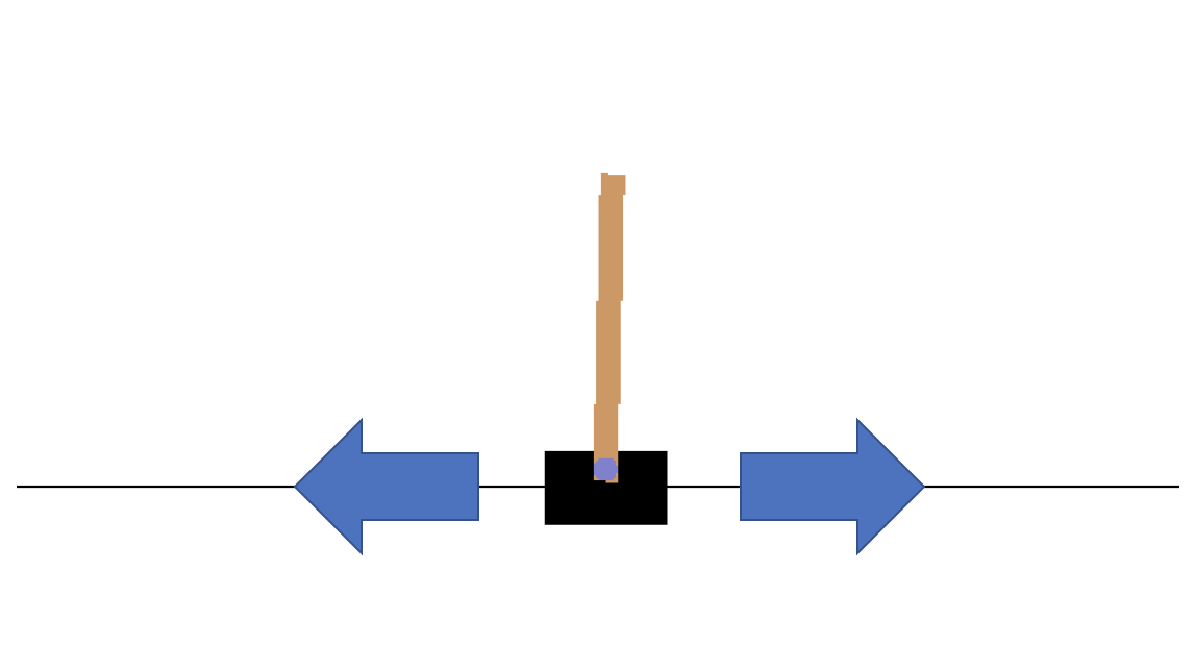
\includegraphics[width=80mm]{images/TsuruokaLab/cartpole.eps}
   \caption{Cart Pole の様子}
   \label{fig:cartpole}
  \end{figure}

  \verb+main.py+の
  \begin{lstlisting}[basicstyle=\ttfamily\footnotesize, frame=single]
   env = gym.make('Easymaze-v0')
  \end{lstlisting}
  を
  \begin{lstlisting}[basicstyle=\ttfamily\footnotesize, frame=single]
   env = gym.make('CartPole-v0')
  \end{lstlisting}
  に変更するだけで,CartPoleを試すことができる.

  \begin{practice}
   CartPoleに対してDQNを学習させ,様子を観察せよ.もし余裕があれば,ローカル環境(学科PCなど)でも試してみるとよい.ローカル環境では,\verb+main.py+の\verb+prints_detail+変数を\verb+True+にすることで,エージェントがCartPoleをプレイする様子を動画で見ることができる.
   ゲームは棒が15度傾いた時点で終わってしまうので,各episodeが一瞬で終わってしまって動画がよくわからないかもしれない.その場合は,\verb+done+が\verb+True+になってもループを抜けずに\verb+env.render()+を続けるようにするとよい.
  \end{practice}

  先述の通り,報酬の最大値は200点である.おそらく,現在のDQNは数十点程度しか取れなかったことだろう.

  \begin{practice}
   CartPoleにおいて,10episodes連続で200点を取ることができるエージェントを作成せよ.
   現在のDQNのどこに問題があるのかを考え・調べ,様々な方法を試してみよ.
  \end{practice}

  例えば,以下のような項目を調べるとよい.
  \begin{itemize}
   \item 隠れ層の大きさや枚数は必要十分か.
   \item 学習率や最適化アルゴリズムは適切か.
   \item 学習のepisode数は十分か.
   \item 過学習を起こしていないか.
   \item 探索の方式は適切か.
   \item Replay bufferは小さすぎないか.
   \item DQNより良いアルゴリズムはないか.
  \end{itemize}

  周りの学生やTAと相談し,できるだけ高得点を取ることのできるエージェントを作ろう.

  \subsection{発展課題・アイディア}

  ここでは,実験後半の自由課題で強化学習を使いたい学生のために,いくつか課題の種を挙げる.これらの課題のうちいずれかを選択してもよいし,これらを基に自由に課題を設定してもらっても構わない.

  \begin{itemize}
   \item OpenAI Gym には,様々なゲームが用意されている.CartPoleのように比較的単純なゲームだけでなく,ビデオゲーム(Atari)や対戦ゲーム(囲碁)などもある.これらのゲームで高得点を得られるエージェントを作ってみよう.その際,1つのゲームに特化するのか,どんなゲームにも適用できるようにするのかは意識するべきである.例えば,今年の6月にはMicrosoftのチームがAtariの ``Ms. Pac-Man''で最高得点である999,990点を取ったと発表した~\cite{allison2017pacman}が,彼らはこのゲームに特化したエージェントを作っており,全く事前知識を用いていないというわけではない.その一方で,DeepMindが発表したDQNは,Atariの49のゲーム全てに全く同じパラメータを用いて学習させ,多くのゲームで人間を超えるスコアを出しているが,すべてのゲームで最高得点を取ったというわけではない.
   \item 強化学習は非常に一般的なモデルであり,現実の様々な問題に適用できるはずである.解決すべき身近な問題を見つけ,強化学習の仕組みに落とし込むことで解決してみよう.制御・最適化などの分野や,自律ロボットの行動などが応用先として有名である.
   \item この実験の他のトピックと組み合わせてみよう.画像分類で強化学習をするとはどういうことだろうか? あるいは,翻訳や要約と強化学習を組み合わせるとどうなるだろうか?
   \item 最新の強化学習の手法を調べ,実装してみよう.まだソースコードが公開されていないなら,実装して世界に公開することで,誰かの役に立てるかもしれない.
   \item ソーシャルゲームや有名なボードゲームなど,身近なゲームを\verb+gym.Env+として実装し,強化学習を適用してみよう.どのようなエージェントが得られるだろうか.
   \item 強化学習の手法を,他の手法と比較してみよう.例えば,強化学習の環境として仮定されているMarkov Decision Processでは,状態遷移規則$T(s, a)\in S$がわかっていれば線形計画法などで解くことができる.また,遺伝的アルゴリズムなどを用いてもエージェントを作ることができる.これらの手法と強化学習の手法との違いはなんだろうか.
   \item 強化学習のエージェントが取れる点数をゲームの「難しさ」だと考えることで,ゲームの難易度調整をしてみよう.例えば,プレイしているうちにだんだんと難易度がユーザにとって最適なものになっていくゲームが作れないだろうか?
   \item 2017年10月19日にGoogle DeepMindが強化学習で(人間の棋譜を用いずに)囲碁の強いエージェントを作ることに成功したと発表した (\url{https://deepmind.com/blog/alphago-zero-learning-scratch/}).この論文を読み,AlphaGo Zeroがどのようにして学習を行っているのかを理解し,まとめてみよう.OpenAI Gymの枠組みでAlphaGo Zeroは実装できるだろうか? もしできないとしたら,それはなぜか?
  \end{itemize}
